% \vspace{-0.1in}
\section{Evo-ROS Framework}
\label{s:evoros}

\xpkm{This section will provide details on the Evo-ROS framework, but (for the double-blind review)
as if it is a tool we pulled off the Internet and installed on our systems.}

\xpkm{Much of the rest of this section can be adapted from Section 2 (Technologies) 
of your term project report,
except for the details of the Erle-rover simulation, which will be discussed in 
Section~\ref{s:rover}.
We should also include a Figure of the interworkings of Evo-ROS.
I like Figure 3 from your report, though we might need}

\begin{comment}
%%%%%%%%%%%%%%%%%%%%%%
This study employs four main software packages: the Robot Operating System (ROS)~\cite{ROS.main}, Gazebo~\cite{Gazebo.main}, Ardupilot~\cite{Ardupilot.main}, and Evo-ROS. 
%
ROS, Gazebo, and Ardupilot emulate the typical software stack used in in commercial robot design and real-world situations. 
%
ROS is a flexible framework for writing robot controllers consisting of tools, libraries, and conventions that simplify the task of creating complex and robust behavior across a wide variety of robotic platforms. 
%
ROS is commonly used in the manufacturing industry and robotics research.  
%
Controllers are capable of operating robots across diverse platforms such as robotic arms, aerial drones, and UGVs. 
%
Here, ROS is used to implement an obstacle avoidance algorithm for the UGV.
%%%%%%%%%%%%%%%%%%%%%%

%%%%%%%%%%%%%%%%%%%%%%
Simulations are conducted using Gazebo, chosen for its support of complex environments, extensive libraries of simulated sensors modeled after commercially available devices, and the strong coupling with ROS. 
%
Furthermore, Gazebo natively supports ROS code, allowing the same control code to be used in simulation or on the physical UGV.
%
% This statement is too strong, unless we have a supporting reference.
%With these capabilities that Gazebo offers, the reality gap between what is observed in simulation and the behavior of a physical system should be minimal.
%%%%%%%%%%%%%%%%%%%%%%

%%%%%%%%%%%%%%%%%%%%%%
Ardupilot is an advanced, full-featured, and reliable open-sourced autopilot software capable of controlling a wide variety of vehicle systems including rovers, airplanes, multi-rotors, helicopters, boats, and submarines. 
%
Ardupilot has built-in algorithms for the waypoint following task examined in this study.  
%%%%%%%%%%%%%%%%%%%%%%

%%%%%%%%%%%%%%%%%%%%%%
Together, ROS, Gazebo, and Ardupilot produce a robust simulation environment that emulates the operating state a physical UGV will encounter.  
%
The simulated rover is exposed to representations of physical environments that a physical UGV would operate in. % 
However, these software packages are traditionally employed in simulations wherein an experimenter manually configures behaviors and configurations of the robot platform.   
%
Such a process is unsuitable for evolutionary search as many simulations need to be conducted in an automated manner.  
%%%%%%%%%%%%%%%%%%%%%%
\end{comment}

The Evo-ROS framework is intended as a bridge between the evolutionary robotics community and the broader field of robotics.  
Evo-ROS integrates evolutionary algorithms with evaluations constructed using
popular software tools: ROS, Gazebo and, for the case study here, Ardupilot.
ROS~\cite{ROS.main} is a publisher/subscriber framework for writing robot control software 
and includes a large collection of libraries realizing
complex interactions among communicating components.
Here, ROS is used to implement an obstacle avoidance algorithm for the UGV.
%%%%%%%%%%%%%%%%%%%%%%
The Gazebo simulator~\cite{Gazebo_paper_ref}
includes models for a wide variety of commercial devices and 
enables the same control code to be used in both simulated and physical robots.
%%%%%%%%%%%%%%%%%%%%%%
Ardupilot~\cite{Ardupilot.main} is an open-source autopilot stack 
capable of controlling terrestrial, aquatic and aerial vehicles.
Ardupilot has built-in algorithms 
for the waypoint following task addressed in this study.  
%%%%%%%%%%%%%%%%%%%%%%

%%%%%%%%%%%%%%%%%%%%%%

Together, ROS, Gazebo, and Ardupilot can produce a simulation
of commercial robots operating in complex physical environments.
% such as those in which 
% simulation
% environment that emulates the operating state a physical UGV will
% encounter.
% 
% %
% 
% The simulated rover is exposed to representations of physical
% environments that a physical UGV would operate in.
% 
However, these software packages are traditionally used 
during robot development to test new designs manually configured by the experimenter.
%
Moreover, they typically simulate the target platform at real-time speed,
often interacting with a user through a remote control interface identical
to that used with the corresponding physical platform.
%
\xgas{Not sure if this is the place to introduce MAVROS}
\xpkm{Agreed.  Let's put it later.}\xgas{MAVROS is a packaged communication driver that enables ROS processes to communicate to various autopilots, including Ardupilot, by converting messages to follow the MAVLink protocol.}
\xjmm{My thought is that MAVROS muddies the water.  It is not necessary to understand the basic control flow.}
% 
Such a process is unsuitable for evolutionary search, where large numbers of 
simulations need to be conducted in an automated manner and, typically, much
faster than real time.

%%%%%%%%%%%%%%%%%%%%%%


\paragraph{Evo-ROS Structure}
%%%%%%%%%%%%%%%%%%%%%%
Evo-ROS
comprises a set of ROS processes capable of spawning, managing, and changing simulations
carried out by the software tools described above.
%
Specifically, Evo-ROS defines the 
interface between an external evolutionary algorithm (a GA in the present study) and the simulation environment,
enabling individuals from the GA population to be evaluated within the ROS/Gazebo/Ardupilot
stack. 
%
A user would need to construct the genome for their specific problem, and integrate with the provided GA code.  
%
In a typical evolutionary run, multiple Evo-ROS instances are executed
in parallel across virtual machines (VMs).
% 
This configuration 
enables the large number of simulations required for a typical evolutionary run.
% Reality gap comments here are again a bit too strong.  I toned it down a bit, unless we have a citation.
% Ultimately, this combination of software aims to a) 
% utilize a robust, high-performance simulation environment typically employed in the robotics community and B) allowing for the evolved controller code to be directly transferred to a physical UGV.
% %%%%%%%%%%%%%%%%%%%%%%

Figure~\ref{evo_ros_diagram} depicts the main components of Evo-ROS and their interaction
for an individual evaluation.
%
The Evo-ROS ``core'' consists of three main components: 
the transporter, software manager, and the simulation manager. 
%
The transporter is responsible for maintaining communication between an instance of Evo-ROS and the external GA via TCP sockets. 
%
The software manager is responsible for spawning and managing the processes within Evo-ROS, including control~(ROS) and simulation~(Gazebo) software. 
%
A user only has to start the software manager process which then instantiates
all the necessary software (ROS, Gazebo, Ardupilot, etc.).
% 
% \ajc{Doesn't the user also need to write and start an external EA?}
%
The simulation manager monitors various aspects of 
an individual Gazebo simulation, as discussed below.  
%
% \gas{added next 3 sentences.}
%
The rover is equipped with a ROS-based navigation controller that includes waypoint following and obstacle avoidance modes as well as a mechanism for triggering transitions between these modes.
%
These modes are covered in detail in Section~\ref{s:rover}.
%
For the case study, commands generated by ROS-based controllers are sent via MAVROS to the Ardupilot software running on the rover.  
%
They are then transmitted over a TCP link to the vehicle using the MAVProxy protocol. 
%
% \jmm{
Note: The Ardupilot and MAVROS components can be easily swapped out for other low-level control libraries.
% }
% \gas{Note1: I am good with added Jared's above note to the text. Note2: If we are just using ROS-based control (like with the autorally) the output of the Rover Nav controller could be directly looped back to Gazebo. Completely cutting out Ardupilot and MAVROS components. Not sure if it is worth mentioning or not}  
% JMM: I don't think we should overcomplicate it.  Might lead the reviewers astray.
%

% for example, termination conditions.
%In the case of the UGV simulations in this study, termination conditions
%include successful completion of the assigned mission, a UGV collision with another object, 
%and reaching the end of the allotted evaluation time.
%%%%%%%%%%%%%%%%%%%%%%
\vspace{-0.1in}
\begin{figure}[ht]
	\centering
    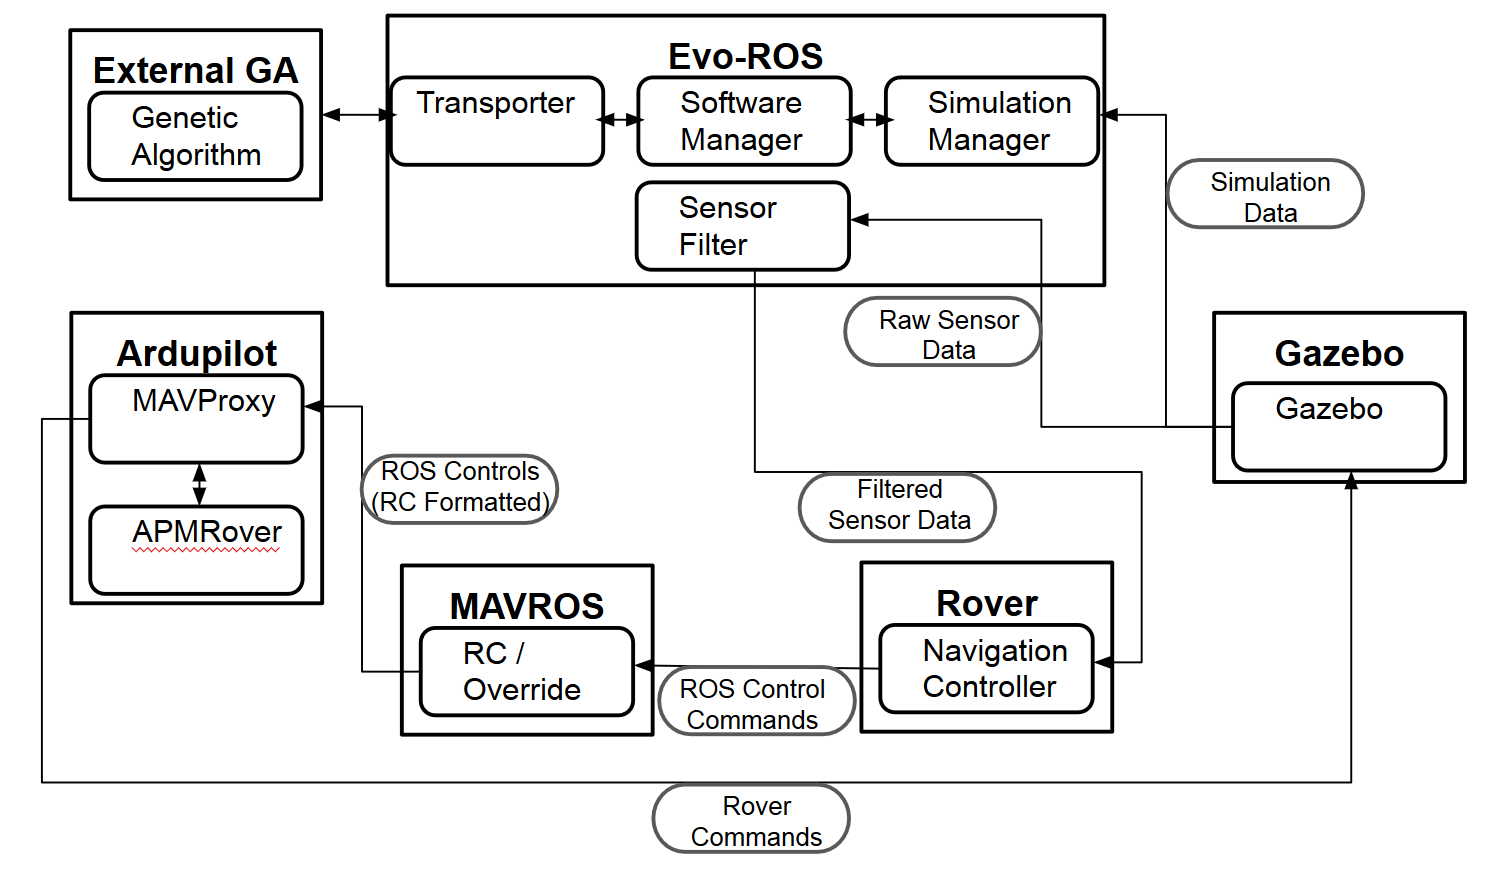
\includegraphics[width=0.47\textwidth]{Figures/evo_ros_diagram.PNG}
    \vspace{-0.05in}
    \caption{Main processes and communication channels 
Evo-ROS management of an individual simulation environment.}
    \label{evo_ros_diagram}
    \vspace{-0.1in}
\end{figure}

%%%%%%%%%%%%%%%%%%%%%%

%%%%%%%%%%%%%%%%%%%%%%

%
%%%%%%%%%%%%%%%%%%%%%%

%%%%%%%%%%%%%%%%%%%%%%
As shown in Figure~\ref{evo_ros_diagram},
an additional component, the sensor filter, has
been added to Evo-ROS for this study.
%
% \jmm{
One of our design goals with Evo-ROS is to allow simple integration of specific components.  The sensor filter is
% }
%
%The sensor filter is a 
a lightweight process that intercepts raw sensor data from Gazebo
and applies filters to the data before forwarding it to the UGV controller. 
%
This filtering could involve injecting noise into sensor readings, introducing delay between when the data is read in Gazebo and delivered to the controller, or selectively neglecting to forward data so that the controller does not receive the readings from specified sensors. Filtering  enables simulating sensor failures in the case study described later.
\xpkm{Hmm, I do not understand what this means.  Further explanation/example?}
\xjmm{I don't think we need this paragraph.  It again muddies the overall message, and how we remove sensor information is not really necessary.  We state that we damage one or more sensors removing it from the pool, and move on.  That has been stated elsewhere.}
%%%%%%%%%%%%%%%%%%%%%%

\begin{figure*}[!htb]
    \centering
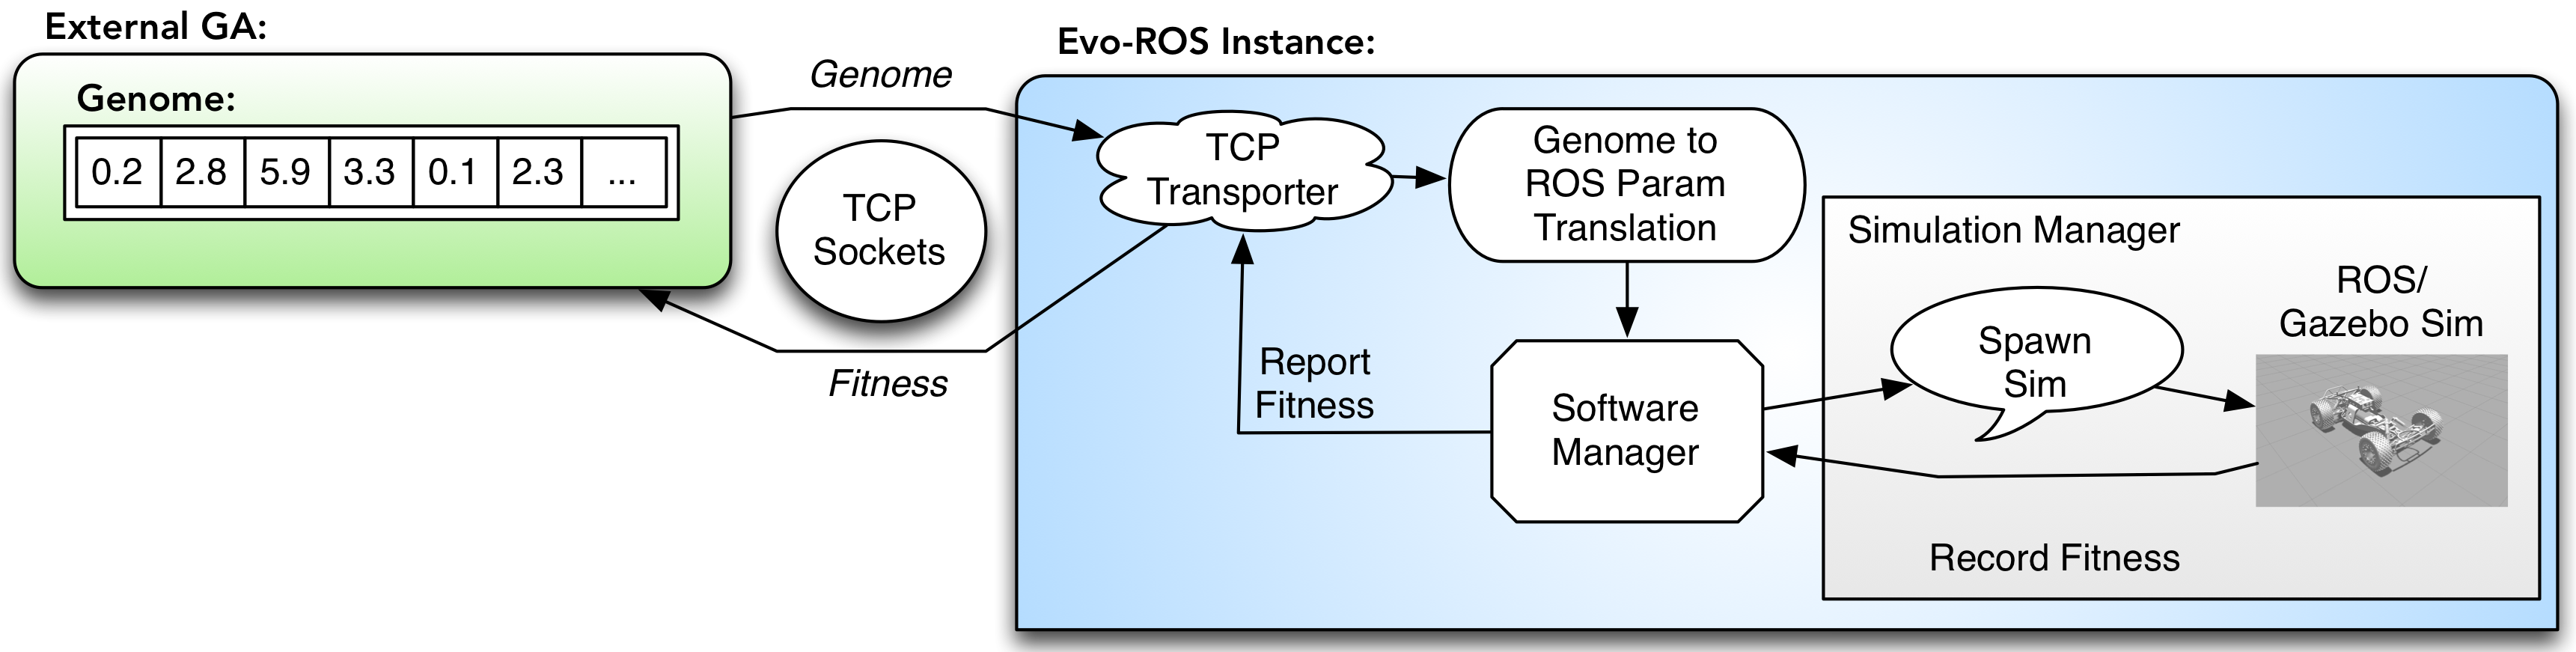
\includegraphics[width=6.25in]{./Figures/Workflow.png}
\vspace{-0.075in}
\caption{The workflow of evaluating an individual genome using an Evo-ROS instance.}
\label{fig:workflow}
\vspace{-0.1in}
\end{figure*}

% \begin{figure}[!htb]
%     \centering
% 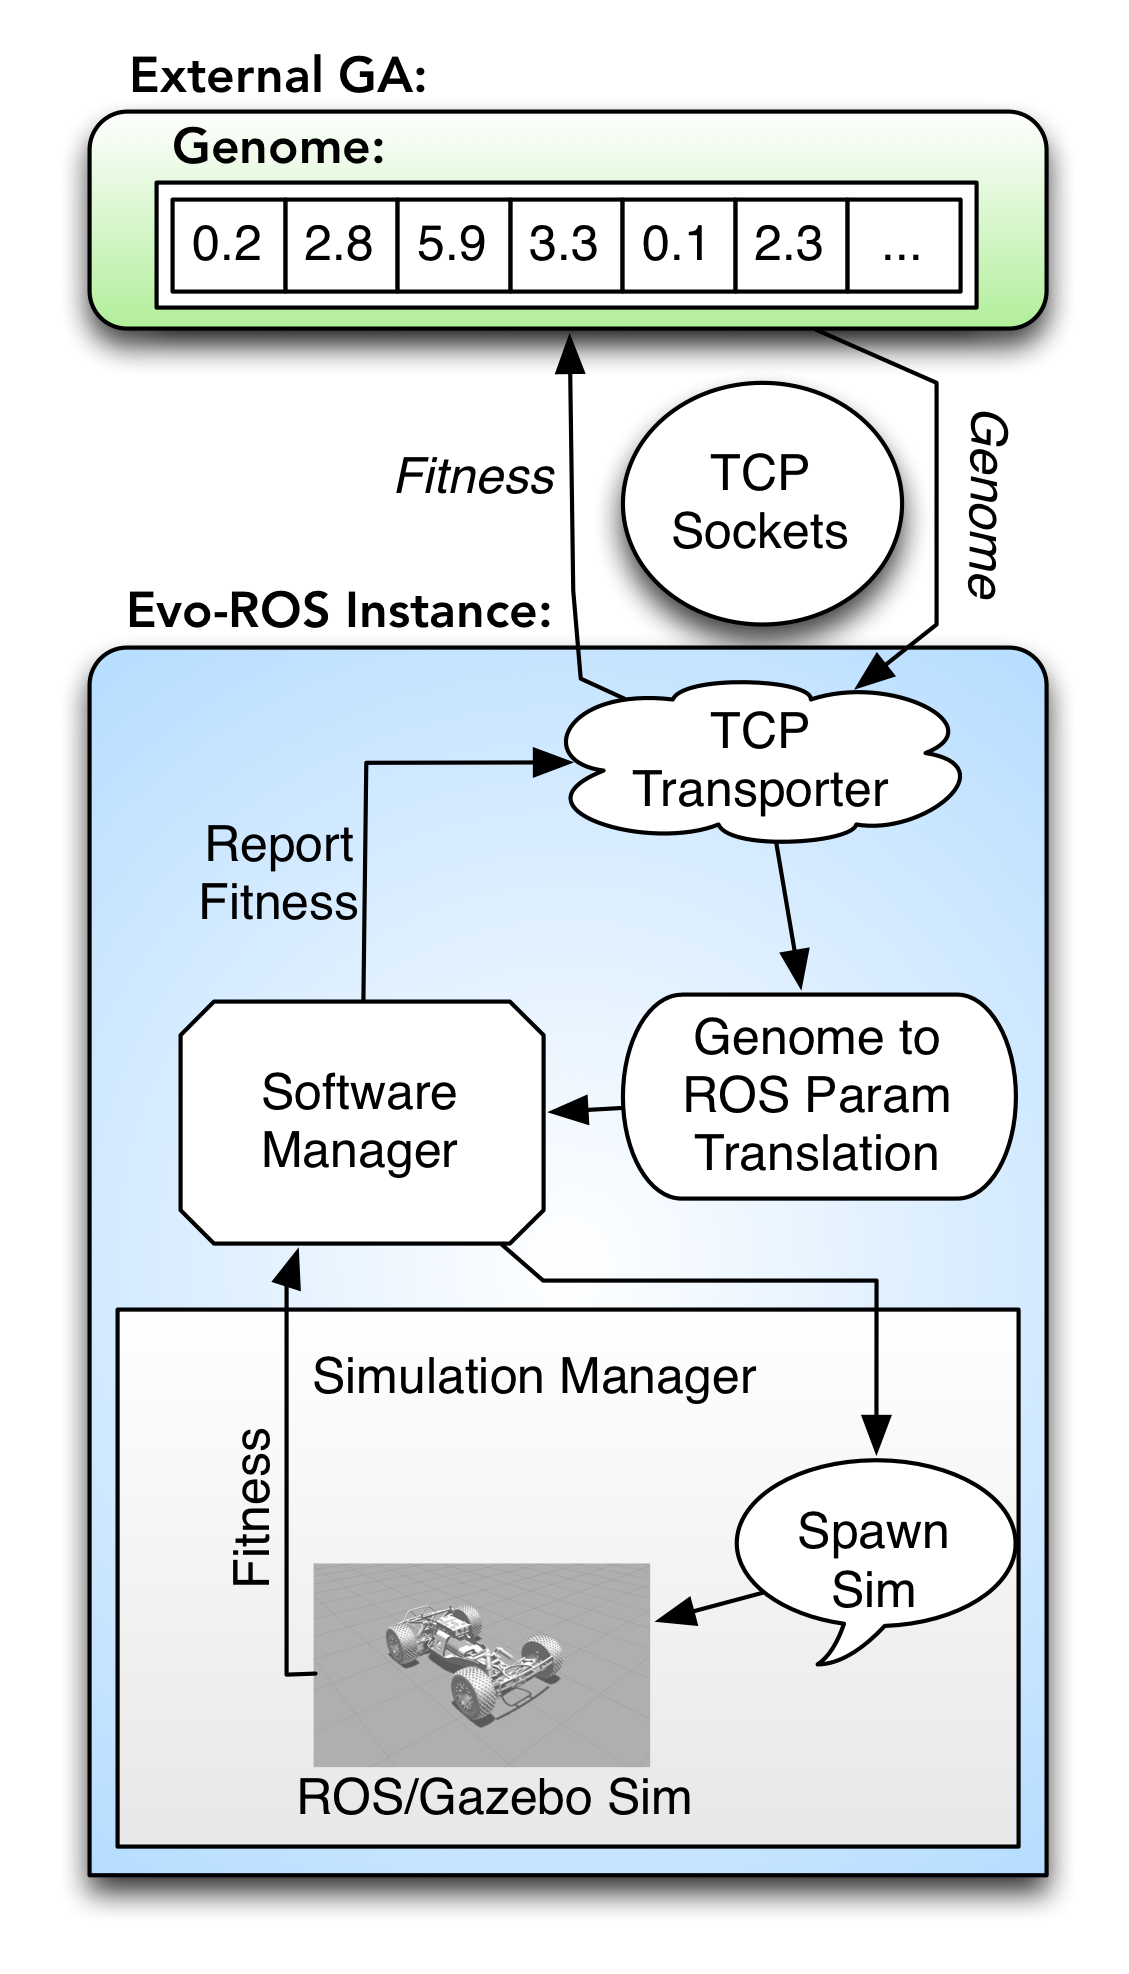
\includegraphics[width=3.5in]{./Figures/Workflow_Sin_Col.png}
% \caption{The workflow of evaluating an individual genome using an Evo-ROS instance.}
% \label{fig:workflow}
% \end{figure}

%%%%%%%%%%%%%%%%%%%%%%
\vspace{-0.1in}
\paragraph{Evo-ROS Workflow}
%
Figure~\ref{fig:workflow} depicts the workflow of evaluating an individual.
% 
First, the GA encodes the attributes of the individual in a genome.
Attributes of an individual could be either behavioral, such as parameter values for various controllers, or physical, such as the number, type, or location of sensors with which this individual is equipped. 
\xpkm{expand on example attributes?}
\xjmm{Wait for the GA section?  Forward reference it?}
%
The genome is transferred via a TCP connection to the transporter process within a single Evo-ROS  instance. 
%
Once received, controller parameters and physical traits from the genome are 
transformed into corresponding ROS parameters.  
%
The transporter then sends a ready flag, via the appropriate ROS topic interface,
to the software manager process. 
%
The software manager determines whether a new simulation environment needs
to be spawned or if the previous one can simply be reset. 
%
(To reduce overhead, 
when evolving controller parameters with unchanging physical traits, the simulation process is persistent and only needs to
be reset before starting a new evaluation.
%
However, when physical traits of the robot are being changed,
such as evolving sensor placements, the software manager
must tear down the simulation environment and modify the robot's
unified robot description format (URDF) model file to reflect the
changes.)
%
The software manager then
spawns the various simulation components, as described above, as well as 
a simulation manager process, and waits for each to initialize.
% simulationThe software manager then spawns all of the software
% applications required for the simulation environment (a ROS
% launch file, a ROS based vehicle controller, Ardupilot, and
% Gazebo), along with 
%
It then hands control to the simulation manager and 
waits until the simulation session completes.

The simulation manager handles an individual evaluation in the physics simulation.  
%
It monitors information within both ROS and Gazebo, including several
metrics describing the state of the simulation.
In this study, such metrics include the speed of travel, 
progression through the mission, distance to each waypoint, collisions with any objects, 
termination conditions (successful completion of the mission, 
reaching the end of the allotted evaluation time).
% as termination conditions.
%
% These could include the UGV colliding with another object, the assigned mission being completed, or if the mission wasn't able to be completed in the alloted amount of time. 
% %
At the conclusion of an evaluation, the simulation manager reports 
the performance of the individual to the software manager. 
%
The software manager forwards the performance report to the transporter, 
which relays it to the GA for calculating fitness.
\xpkm{Figure shows fitness reported by software mgr.  See my email regarding the figure.}
The software manager then cleans up the simulation environment.
This process is repeated for each individual sent to the Evo-ROS instance.
%%%%%%%%%%%%%%%%%%%%%%

%%%%%%%%%%%%%%%%%%%%%%
\paragraph{Current Limitations}
A limiting factor of the Evo-ROS framework using the Ardupilot control framework is the fact that simulations must be capped at near real-time due to the integral 400Hz update loop in the Ardupilot stack.  
%
Furthermore, due to the distributed nature of the ROS system, individual processes within a single ROS instance communicate through a socket-based architecture.  
%
Typically, this means that only a single ROS/Gazebo instance can be run on one physical machine.  
%
We address this issue by creating an individual virtual machine (VM) for each ROS/Gazebo instance and
extend the communication ``fabric'' to include a pool of VMs running on a cluster of
physical nodes.
%
% Therefore, parallelization is required to best utilize computing resources.
%%%%%%%%%%%%%%%%%%%%%%

%%%%%%%%%%%%%%%%%%%%%%
Figure~\ref{evo_multiple} illustrates
our parallelization strategy.
%
Each Evo-ROS instance communicates with the external GA through the transporter process.
%
Instances of Evo-ROS are spawned on multiple VMs spread across several physical machines. 
%
This configuration allows the population of 
the GA to be distributed across many identical simulation environments,
greatly reducing the overall evaluation time per generation.
%
The limiting factor is the number of individual VMs that can be 
spawned across a compute cluster.
%%%%%%%%%%%%%%%%%%%%%%
%\vspace{-0.1in}
\begin{figure}[ht]
	\centering
    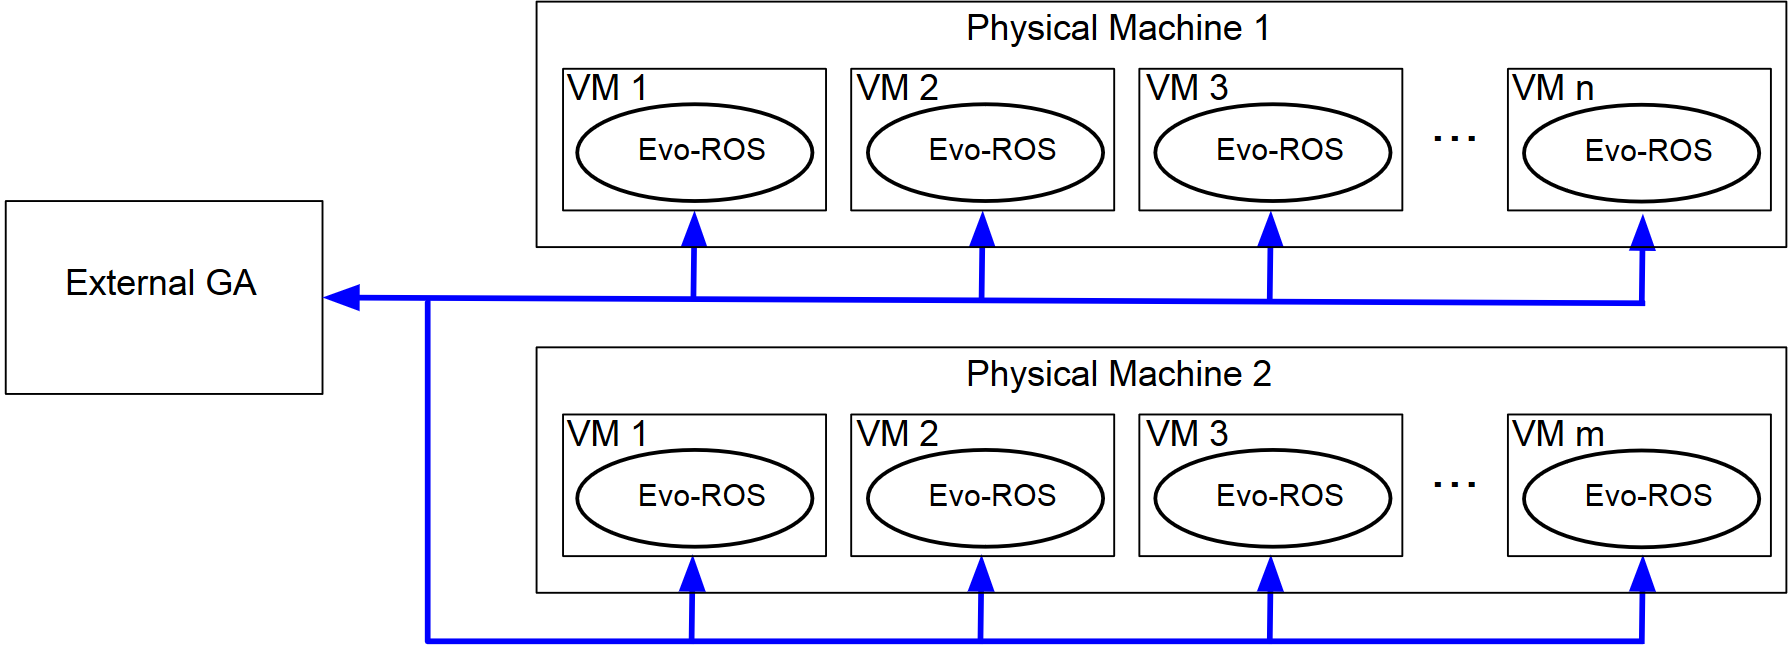
\includegraphics[width=0.45\textwidth]{Figures/evo_ros_distro_setup.PNG}
    \caption{Parallelization of evaluations in Evo-ROS.}
    \label{evo_multiple}
    \vspace{-0.1in}
\end{figure}

